\documentclass[10pt]{article}\usepackage[]{graphicx}\usepackage[]{color}
%% maxwidth is the original width if it is less than linewidth
%% otherwise use linewidth (to make sure the graphics do not exceed the margin)
\makeatletter
\def\maxwidth{ %
  \ifdim\Gin@nat@width>\linewidth
    \linewidth
  \else
    \Gin@nat@width
  \fi
}
\makeatother

\definecolor{fgcolor}{rgb}{0.345, 0.345, 0.345}
\newcommand{\hlnum}[1]{\textcolor[rgb]{0.686,0.059,0.569}{#1}}%
\newcommand{\hlstr}[1]{\textcolor[rgb]{0.192,0.494,0.8}{#1}}%
\newcommand{\hlcom}[1]{\textcolor[rgb]{0.678,0.584,0.686}{\textit{#1}}}%
\newcommand{\hlopt}[1]{\textcolor[rgb]{0,0,0}{#1}}%
\newcommand{\hlstd}[1]{\textcolor[rgb]{0.345,0.345,0.345}{#1}}%
\newcommand{\hlkwa}[1]{\textcolor[rgb]{0.161,0.373,0.58}{\textbf{#1}}}%
\newcommand{\hlkwb}[1]{\textcolor[rgb]{0.69,0.353,0.396}{#1}}%
\newcommand{\hlkwc}[1]{\textcolor[rgb]{0.333,0.667,0.333}{#1}}%
\newcommand{\hlkwd}[1]{\textcolor[rgb]{0.737,0.353,0.396}{\textbf{#1}}}%
\let\hlipl\hlkwb

\usepackage{framed}
\makeatletter
\newenvironment{kframe}{%
 \def\at@end@of@kframe{}%
 \ifinner\ifhmode%
  \def\at@end@of@kframe{\end{minipage}}%
  \begin{minipage}{\columnwidth}%
 \fi\fi%
 \def\FrameCommand##1{\hskip\@totalleftmargin \hskip-\fboxsep
 \colorbox{shadecolor}{##1}\hskip-\fboxsep
     % There is no \\@totalrightmargin, so:
     \hskip-\linewidth \hskip-\@totalleftmargin \hskip\columnwidth}%
 \MakeFramed {\advance\hsize-\width
   \@totalleftmargin\z@ \linewidth\hsize
   \@setminipage}}%
 {\par\unskip\endMakeFramed%
 \at@end@of@kframe}
\makeatother

\definecolor{shadecolor}{rgb}{.97, .97, .97}
\definecolor{messagecolor}{rgb}{0, 0, 0}
\definecolor{warningcolor}{rgb}{1, 0, 1}
\definecolor{errorcolor}{rgb}{1, 0, 0}
\newenvironment{knitrout}{}{} % an empty environment to be redefined in TeX

\usepackage{alltt}
\usepackage{mathpazo}
\usepackage[breaklinks=true]{hyperref}
\usepackage{url}
\usepackage[a4paper,margin=1.5cm]{geometry}
\usepackage{a4wide}
\usepackage{float}
\usepackage[english]{babel}
\usepackage[utf8]{inputenc}
\usepackage{amsmath}
\usepackage{amssymb}
\usepackage{color}
\usepackage[backend=bibtex,style=numeric-comp,sorting=none]{biblatex}
\bibliography{report}
\usepackage{subcaption}
\usepackage[font={small}]{caption}
\usepackage{booktabs}
\usepackage{listings}
\usepackage{tikz}
\usetikzlibrary{decorations, matrix, arrows, shapes, positioning, calc, fit}
\tikzset
{
  mybox/.style={draw, minimum height=.8cm, minimum width=.9cm},
  myflip/.style={draw, fill=gray!30, minimum height=.8cm, minimum width=.9cm},
  myint/.style={draw, minimum height=.8cm, minimum width=1.1cm},
  mynone/.style={draw=none}
}

\usepackage{graphicx,epstopdf}
\epstopdfsetup{update} % only regenerate pdf files when eps file is newer
\usepackage{cleveref}
\usepackage{collcell} % loads array
\newcolumntype{m}{>{$} r <{$}}
\newcolumntype{u}{>{$[\collectcell\si} l <{\endcollectcell]$}}
\newcommand{\approxtext}[1]{\ensuremath{\stackrel{\text{#1}}{=}}}
\newcommand{\matr}[1]{\mathbf{#1}}
\newcommand{\partt}[2]{\ensuremath{\dfrac{\partial {#1}}{\partial {#2}}}}
\renewcommand{\d}[1]{\ensuremath{\operatorname{d}\!{#1}}} % non-italized differentials
\newcommand{\h}[0]{\ensuremath{\hbar}} % hbar
\newcommand{\qed}[0]{\ensuremath{\tag*{$\square$}}} % QED square
\def\changemargin#1#2{\list{}{\rightmargin#2\leftmargin#1}\item[]}
\let\endchangemargin=\endlist 
\usepackage{amsthm}
\theoremstyle{plain}
\newtheorem{thm}{theorem} % reset theorem numbering for each chapter
\theoremstyle{definition}
\newtheorem{defn}[thm]{definition} % definition numbers are dependent on theorem numbers
\newtheorem{exmp}[thm]{example} % same for example numbers
\renewcommand{\theequation}{\thesection.\arabic{equation}}
\def\changemargin#1#2{\list{}{\rightmargin#2\leftmargin#1}\item[]}
\let\endchangemargin=\endlist    
\newcommand{\ts}{\textsuperscript} 
\title
{
  \phantom{a}\vspace{2cm}
	\textbf
	{
      Genome Informatics: Assignment 1
  }\\[1em]
  \small{University of Cambridge}
}

\author{Henrik Åhl}
\date{\today}

% Stephen's stuff
\newcommand{\R}{\texttt{R}}
\newcommand{\Rfunction}[1]{{\texttt{#1}}}
\newcommand{\Robject}[1]{{\texttt{#1}}}
\newcommand{\Rpackage}[1]{{\mbox{\normalfont\textsf{#1}}}}
\usepackage{xcolor}
\definecolor{Red}{rgb}{0.7,0,0}
\definecolor{Blue}{rgb}{0,0,0.8}
\hypersetup{%
  pdfusetitle,
  bookmarks = {true},
  bookmarksnumbered = {true},
  bookmarksopen = {true},
  bookmarksopenlevel = 2,
  unicode = {true},
  breaklinks = {false},
  hyperindex = {true},
  colorlinks = {true},
  linktocpage = {true},
  plainpages = {false},
  linkcolor = {Blue},
  citecolor = {Blue},
  urlcolor = {Red},
  pdfstartview = {Fit},
  pdfpagemode = {UseOutlines},
  pdfview = {XYZ null null null}
}
%% Listings
\lstset{ 
  language=R,                     % the language of the code
  basicstyle=\footnotesize,       % the size of the fonts that are used for the code
  numbers=left,                   % where to put the line-numbers
  numberstyle=\tiny\color{gray},  % the style that is used for the line-numbers
  stepnumber=1,                   % the step between two line-numbers. If it's 1, each line will be numbered
  numbersep=5pt,                  % how far the line-numbers are from the code
  backgroundcolor=\color{white},  % choose the background color. You must add \usepackage{color}
  showspaces=false,               % show spaces adding particular underscores
  showstringspaces=false,         % underline spaces within strings
  showtabs=false,                 % show tabs within strings adding particular underscores
  rulecolor=\color{black},        % if not set, the frame-color may be changed on line-breaks within not-black text (e.g. commens (green here))
  tabsize=2,                      % sets default tabsize to 2 spaces
  captionpos=b,                   % sets the caption-position to bottom
  breaklines=true,                % sets automatic line breaking
  breakatwhitespace=false,        % sets if automatic breaks should only happen at whitespace
  title=\lstname,                 % show the filename of files included with \lstinputlisting;
                                  % also try caption instead of title
  keywordstyle=\color{blue},      % keyword style
  commentstyle=\color{green},   % comment style
  stringstyle=\color{purple},      % string literal style
  escapeinside={\%*}{*)},         % if you want to add a comment within your code
  morekeywords={*,...}            % if you want to add more keywords to the set
} 
\usepackage{verbatim}
\usepackage{multicol}
\usepackage{float}
\def\changemargin#1#2{\list{}{\rightmargin#2\leftmargin#1}\item[]}
\let\endchangemargin=\endlist
\IfFileExists{upquote.sty}{\usepackage{upquote}}{}
\begin{document}

\date{\today}
\maketitle
\thispagestyle{empty}

\newpage
\setcounter{page}{1}
\begin{abstract}
\begin{changemargin}{-.8cm}{-.8cm}
{\bf
The current pace of development for \textit{Next Generation Sequencing} (NGS) has allowed for a rapid decrease in cost for genome sequencing from short-read data. Naturally, this provides a high increase in the amount of data available for analysis, which subsequently can aid in understanding the complex patterns and dependencies of the genome on a nucleotide level. More specifically, the amount of data provides a firm basis for novel gene detection and comparison between species.

\hspace{.5cm}In this report, Illumina HiSeq sequencing has been performed on an unknown bacterial sample, which we assemble using the \textbf{Velvet} \textit{de novo} assembler, developed by Zerbino and Berney~\cite{Zerbino08}. The assembled product is identified and compared by alignment to bacterial model organism \textit{Escherichia coli} (E.\ coli). 

\hspace{.5cm}We find that the species, identified as \textit{Buchnera Aphidicola} in \textit{Cinara cedri} (BCc), contains a significantly lower amount of overall genes, and likewise a smaller genome than E.\ coli. However, a large portion of the BCc sample is present in the E.\ coli genome, implying that the BCc genome consists to a larger extent of genes strictly necessary for survival. 
}
\end{changemargin} 
\end{abstract}

\begin{multicols}{2}
\section*{Preface}
This is an assignment report in connection to the \textit{Genome Informatics} module in the Computational Biology course at the University of Cambridge, Michaelmas term 2016. All related code is as of \date{\today} available on \url{https://github.com/supersubscript/compbio/tree/master/src/sp_assignments/assignment_1/}, or available per request by contacting \href{mailto:hpa22@cam.ac.uk}{hpa22@cam.ac.uk}. Likewise, the corresponding assignment can be found on \url{https://github.com/supersubscript/compbio/tree/master/general/gi_assignment_1.pdf}.

\section{Introduction}
\textit{Buchnera Aphidicola} is a bacterial obligate endosymbiont found primarily in connection to aphids. It contains one of the smallest known genomes of living organisms, hosting around 422000 base pairs and 400 genes. However, the genome is also one of the most genetically stable~\cite{Silva2003176}. 

The Buchnera Aphidicola strain found in aphid \textit{Cinara cedri} (henceforth abbreviated BCc) was at the point of sequencing found to be roughly 200 kilobases smaller than other sequenced B.\ Aphidicola strains, furthering the notion that the species and its various strains are undergoing a genome reduction process over time~\cite{2006Perez}. In particular, B.\ Aphidicola is known to lack the genes necessary for production of lipopolysaccharides for its outer membrane, which is done by gene rfaS in related species \textit{Escherichia coli} K-12~\cite{shigenobu2000genome}. Notably, BCc also lacks most metabolic functions, is largely unable to supply for its own nutritional needs, and relies heavily on its symbiotic status in order to survive. The species thus forms an interesting model organism for studying the process of genome reduction and the possibility of a lower threshold of genes required for prolonged existence. It has, however, been hypothesised that the bacterium with its continuing genome evolution is destined for future replacement by another endosymbiont in its aphid host~\cite{2006Perez}.

By use of the Velvet assembler for \textit{de novo} short read sequencing, we assemble our bacterial sample under a range of various configurations of k-mer lengths, ultimately choosing the parameter configuration which renders the best N50 score for future investigations. We utilise this choice to go into a more fine-grained analysis by finding the optimal cut-off lengths and our estimated coverage, consequently attaining our optimised assembly. The genome is then identified and compared to E.\ coli with respect to genomic qualities such as gene number and gene similarities. Finding that the genomes are considerably unlike each other, we pinpoint differences and their possible causes. Finally, we perform an enrichment analysis on common genes, thereby determining their biological functions. 

\section{Methods and Results}
We perform the initial assembly by running Velvet on a set of different k-mer lengths. Our data consist of roughly 1129000 reads of paired-end data of length 100, with an average read-length of ca.\ 500 base pairs. Investigating k-mer lengths between 17--31 in size, with an expected coverage of length 22, we find that the N50 score reaches a maximum at a k-mer length of 25, as can be seen in \cref{fig:kmers}. As we want to exclude the nodes which likely are due to mutations, we want to trim our assembly for low-coverage data points. We also want to set the expected coverage to the number of times we expect each subsequence to be covered, as it allows us to exclude repeats.
\begin{minipage}{0.45\textwidth}
\begin{knitrout}
\definecolor{shadecolor}{rgb}{0.969, 0.969, 0.969}\color{fgcolor}
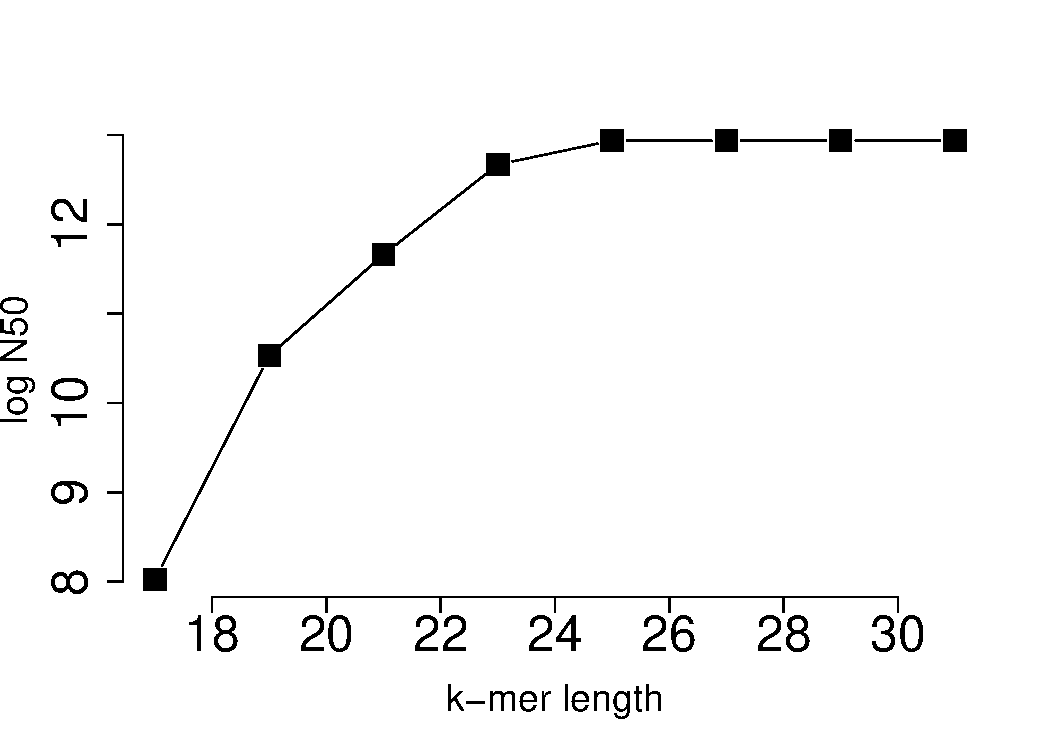
\includegraphics[width=\maxwidth]{figure/unnamed-chunk-1-1} 

\end{knitrout}
\captionof{figure}{N50 distribution for different k-mer lengths.}
\label{fig:kmers}
\end{minipage}
\vspace{.5em}

Given this, we perform another assembly with k-mer length 25, without cut-off. The outcome of this can be seen in \cref{fig:cov,fig:cov_norm}. Noting that there is a bias towards sub-20 coverage in the non-normalised case, and a grouping of length-adjusted coverage nodes in the sub-6 region, we choose to disregard these nodes and repeat the process. Ultimately, we find that an expected coverage of 23, along with a coverage cut-off of 19 gives the most sensible assembly, with the highest N50, and a summed contig length of about 439000 base pairs.

\begin{minipage}{.45\textwidth}
\begin{knitrout}
\definecolor{shadecolor}{rgb}{0.969, 0.969, 0.969}\color{fgcolor}
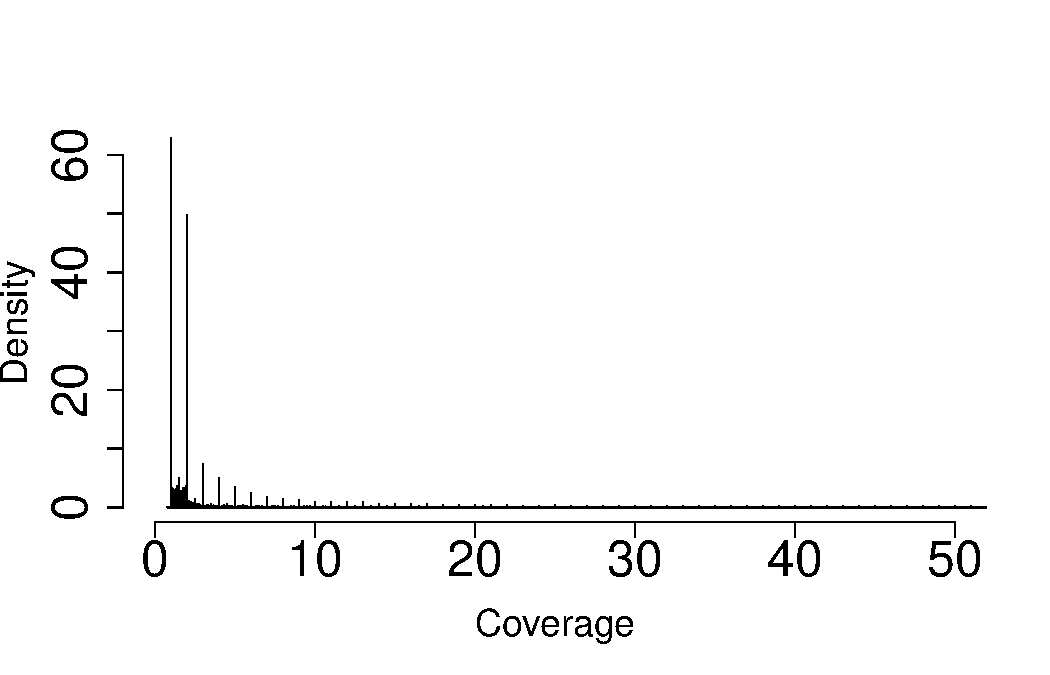
\includegraphics[width=\maxwidth]{figure/COVERAGE-1} 

\end{knitrout}
  \captionof{figure}{Distribution of coverage for non-normalised contigs.}
  \label{fig:cov}
\end{minipage}
\begin{minipage}{.45\textwidth}
\begin{knitrout}
\definecolor{shadecolor}{rgb}{0.969, 0.969, 0.969}\color{fgcolor}
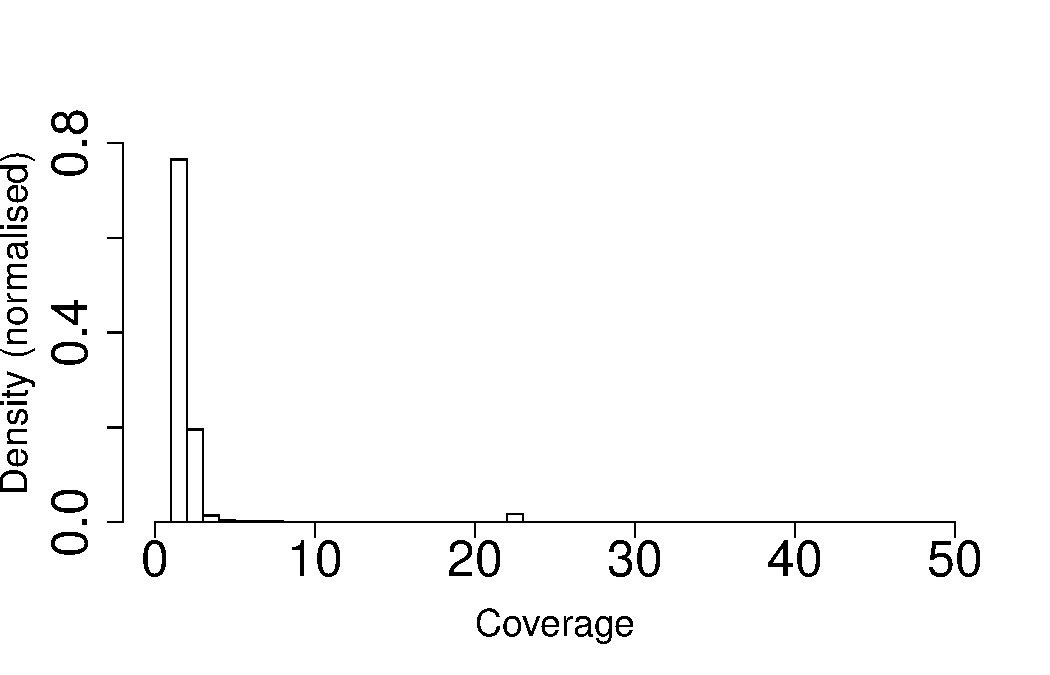
\includegraphics[width=\maxwidth]{figure/COVERAGE_WEIGHTED-1} 

\end{knitrout}
  \captionof{figure}{Coverages for contigs normalised with respect to sequence length. Note how a a group of low-coverage nodes are present also after normalisation, and that some are found in the $> 20$ region. }
  \label{fig:cov_norm}
\end{minipage}
\vspace{.5em}

Using the \textit{NCBI-BLAST} interface to identify the species given our assembly, we indeed find a strong (99~\%) identity correspondence with B.\ Aphidicola in \textit{Cinara cedri}, as well as a 99~\% query cover. For the closest competitor, Buchnera strain \textit{Cinara tujafilina}, the match does not exceed 75~\%, and only reaches a query cover of 31~\% in the local alignment. 

\vspace{-1.5pt}
Retrieving the annotated BCc genes from bacterial genome-portal EnsemblBacteria, we use sequence comparison software Exonerate to align BCc with the closely related species Escherichia coli K-12. Performing a local alignment with affine gaps~\cite{exonerate}, we are able to identify similar genes in the two species. \Cref{tab:exonerate} shows the values extracted from the Exonerate alignment after curation. Note in particular that a large fraction of the BCc gene pool is matched by one or several genes in E.\ coli K-12. Additionally, BCc contains significantly fewer genes overall than the E.\ coli strain. It also finds matches for almost all of its genes, though it should be noted that the local alignment does not account for the overall similarities between genes, but rather included subsequences. In other words, two genes who for example might have similar binding site sequences has a chance of becoming matched in this process. Moreover, the BCc genes find matches for more genes than the number that are shared.
\end{multicols}
\newpage
\begin{table*}
\centering
\caption{Extracted values from Exonerate run for local alignment with affine gap penalties.}
\label{tab:exonerate}
\begin{tabular}{ll}
  \toprule
  \emph{Parameter} & \emph{Value}                     \\\midrule
  Total number of genes in E.\ coli K-12    &	3635    \\
  Total number of genes in BCc	            & 365     \\
  Number of genes in both species	          & 317     \\
  \midrule
  Matched genes in BCc      	              &	350     \\
  Matched genes in E.\ coli K-12            &	759     \\
  Number of matched genes in both species   &	97      \\
  \midrule
  Fraction of BCc genes shared     	        & 0.87    \\
  Fraction of E.\ coli K-12 genes shared	  & 0.09    \\\bottomrule
\end{tabular}
\end{table*}
\begin{multicols}{2}
Also due to the local alignment, it is inevitable that many genes will have several matches, particularly if they contain genomic features which are typical for genes of its given kind. \Cref{fig:matches_bcc,fig:matches_ecoli} shows this phenomenon, where it is evident that some genes are frequently paired with other genes in the corresponding species. For example, the most frequently found E.\ coli gene, rfaS, is matched 293 times, likely due to its relatively long nucleotide sequence. 
\end{multicols}

\begin{figure}[H]
\begin{subfigure}{.49\linewidth}
\begin{knitrout}
\definecolor{shadecolor}{rgb}{0.969, 0.969, 0.969}\color{fgcolor}
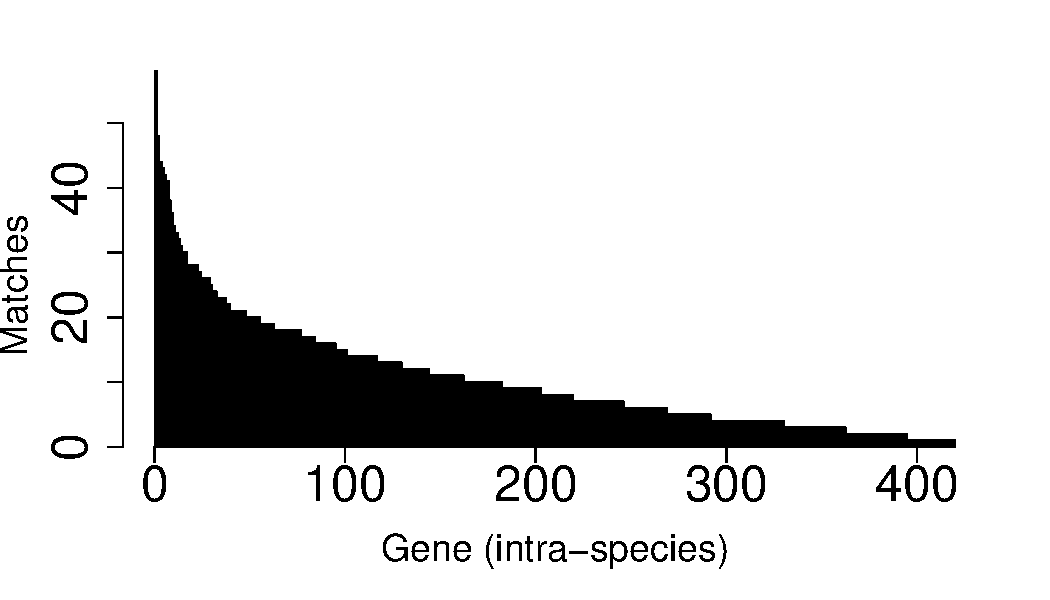
\includegraphics[width=\maxwidth]{figure/unnamed-chunk-2-1} 

\end{knitrout}
\caption{Buchnera Aphidicola in \textit{Cinara cedri}}
\label{fig:matches_bcc}
\end{subfigure}
\begin{subfigure}{.49\linewidth}
\begin{knitrout}
\definecolor{shadecolor}{rgb}{0.969, 0.969, 0.969}\color{fgcolor}
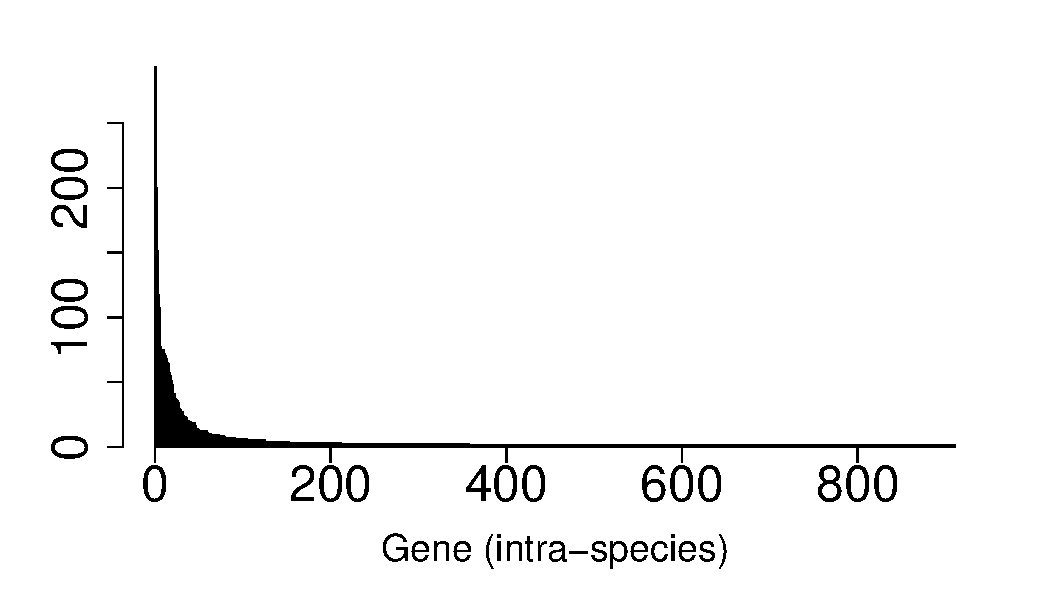
\includegraphics[width=\maxwidth]{figure/unnamed-chunk-3-1} 

\end{knitrout}
\caption{Escherichia coli K-12}
\label{fig:matches_ecoli}
\end{subfigure}
\caption{Number of matches per gene for BCc and E.\ coli K-12 respectively. Note that genes are sorted by number of matches, so that the horizontal position of specific genes differs between the graphs.}
\label{fig:matches}
\end{figure}
\begin{multicols}{2}

The distribution of fraction identity between the alignments is featured in \cref{fig:identity_distribution}. Most alignments have a match fraction around 65~\%, meaning that the differences are mostly fairly big. This stands in relation to the fact that 350  out of the 365 genes in BCc find a corresponding match in the E.\ coli K-12 gene pool. A set of alignments also match with higher accuracy, rendering identity matches of up towards 100~\%. However, these matches mostly consist of shorter subsequences and not necessarily the whole genes. In conclusion, most genes that match between species contain significant differences. 
\begin{minipage}{.45\textwidth}
\begin{knitrout}
\definecolor{shadecolor}{rgb}{0.969, 0.969, 0.969}\color{fgcolor}
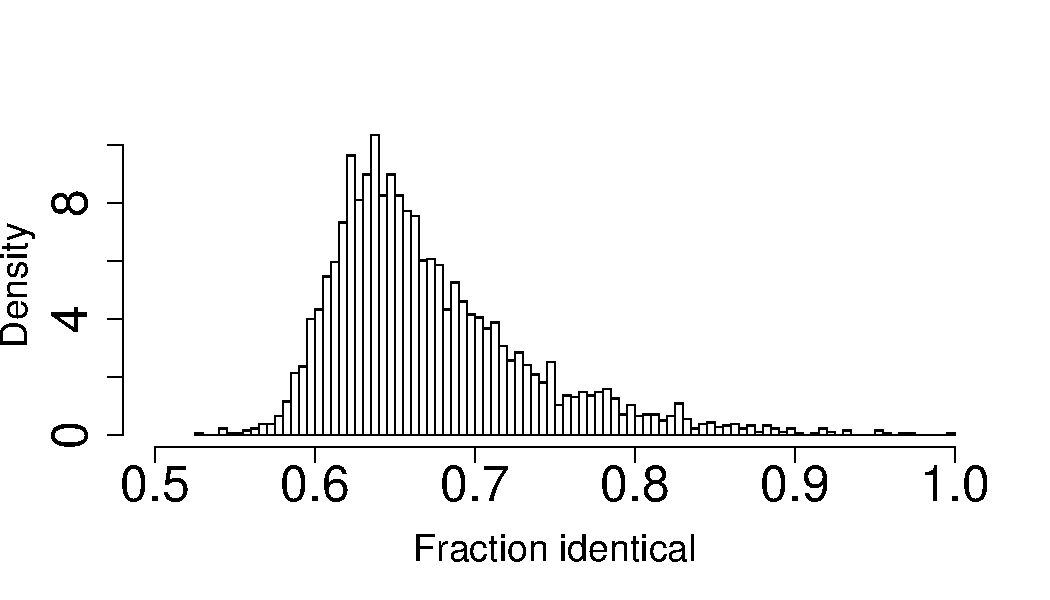
\includegraphics[width=\maxwidth]{figure/unnamed-chunk-4-1} 

\end{knitrout}
\captionof{figure}{Distribution of fraction identity between nucleotide bases between the compared subsequences in the Exonerate local alignment.}
\label{fig:identity_distribution}
\end{minipage}
\vspace{.5em}

\pagebreak Finally, by performing an enrichment analysis on the genes which occur in both species, it is possible to determine which features the species in particular have in common. Using the Gene Ontology (GO) platform, we find that genes overlapping are related in particular to primary metabolic processes, gene expression, translation, various forms of binding, and processes related to maintenance of intra-cellular structures such as organelles. In short, crucial genetic components for living organisms. 

\vspace{-1em}
\section{Discussion}
\subsubsection*{Accuracy in results are limited by the assembly, but marginally so}
Initially, it must by necessity be stated that the results obtained to a slight degree depend on the parameters used for the assembly. The fact that the identification of the species is done by sequence comparison is inherently dependent on our sequenced genome. Still, the fact that such an adequate match is attained in out investigation is reassuring of our method. In more obscure cases it is however a significant limiting factor which ought to be taken into account. In principle, a more systematic approach to reach optimal parameters is clearly favourable, which can be done by performing a more thorough analysis over a larger set of k-mer lengths.

In our particular case, this can of course be seen as a minor problem due to the adequate match of species. Nevertheless, also in the process of identifying the species, we lose some resolution as this is done based on the sequence of the largest assembled contig. This approach is undoubtedly non-stringent, as it completely over-glosses the possibility of novel findings and in practice always relies on partial matching. We can, for example, happen to misidentify more complex sequences as singular, well-known genes or structures. 

In addition to this, using the BLAST interface was here done in a fairly offhanded way. As the typical BLAST alignment relies on heuristic methodics and local alignments, also this forms a procedural speed-bump.

\subsubsection*{Possibly faulty annotations allow for an increase in multiply matched genes}
We are, however, able see even in our rough comparison between the species that indeed many of the genes found in BCc also occur in E.\ coli K-12. Our local alignment hampers the analysis somewhat by rendering multiple matches for many of the genes in both species. In particular in E\. coli K-12, which has a significantly longer genome and larger gene pool, the consequences of this can be clearly seen. The fact that the rfaS gene is matched so frequently is likely due to its known role in the production of lipopolysaccharides -- a capability we recall that the BCc strain lacks. This also raises the issue of annotation, as such a significant amount of genes in BCc match this gene signifies that they may in fact rather be pseudogenes, having arisen as a consequence of the degradation of the genome over time. In contrast, a few genes in the BCc genome are not found at all in E.\ coli K-12, possibly being due to novel genes having developed in a similar fashion.

In E.\ coli, many genes lack matches at all, which plays according to expectations as the BCc genome is considerably smaller. These have likely fallen out under the evolutionary trajectory due to genomic deletions. 

Another possible explanation of genes with multiple matches is that repetitive regions may have been included over several differently annotated genes. Also, as previously mentioned, genes containing common functional subsequences, such as those relating to binding and of certain proteins and the likes, may cause an increase in multiply matching genes. In principle we ought to be able to circumvent these problems by applying a score threshold for the alignment, although with such an approach we obfuscate a significant portion of genomic features which may be of interest, such as our part-wise alignment to rfaS. 

\subsubsection*{Common genes with Escherichia coli K-12 tell of essential processes for survival}
As many of the genes which exist in both the species relate to functions we can largely consider to be essential, it is not far-fetched to infer that the BCc genome has been scraped down to contain mainly genes strictly necessary for its continued existence. However, even though the strain is known to have lost most metabolic functions, many genes still relate to metabolic processes. Many genes also naturally relate to processes in connection to cellular components such as ribosomal structures and the likes, for which it is hard to consider an organism. 

\section{Conclusion}
We have seen that using sophisticated analytical tools for sequence manipulation and comparison, we are able to assemble a genome with high enough accuracy that we can identify the corresponding species. In comparing our result with reference organism E.\ coli K-12, we are able to see previously identified differences and reasons for the genomic difference. We can also infer possible reasons for the structure and general function of the genome of our species.

\section*{Acknowledgements}
A great many thanks to Julian Melgar for no particular reason. Thank you, Julian!

%%%%%%%%%%%%%
% Problems with parameter choice. More thorough? 
% NCBI-BLAST identification: Only known species, ambiguity. Local search, heuristics. 
% Exonerate uses heuristics
% Alignment incomplete (not everything to everything)
% repeats? Explains many matches?
% Applying score threshold problematic -- might miss relevant information
% Why some genes align to severl, some to none?
% Reason for different genes
% Common functionS
%%%%%%%%%%%%%

\printbibliography
\end{multicols}
\appendix
\section{Genes annotated in both species}
\begin{knitrout}
\definecolor{shadecolor}{rgb}{0.969, 0.969, 0.969}\color{fgcolor}\begin{kframe}
\begin{verbatim}
##   [1] thrA thrB thrC dnaK dnaJ rpsT ileS dapB carA carB ksgA leuD leuC leuB
##  [15] leuA ilvI ilvH ftsA ftsZ secA aceE aceF pcnB yadR dapD map  rpsB tsf 
##  [29] pyrH frr  yaeT fabZ dnaE proS dnaQ nusB cyoE cyoD cyoC cyoB cyoA bolA
##  [43] clpP clpX lon  ppiD mdlA mdlB dnaX ybaB htpG adk  cysS folD ahpC cspE
##  [57] lipA lipB ybeD holA leuS ybeY miaB glnS fldA ybgI sucA sucB gpmA infA
##  [71] trxB serS serC aroA rpsA asnS ompA yccK yceA rluC rpmF fabD fabG acpP
##  [85] holB ycfH mfd  trmU minE minD minC ychF pth  prsA prfA ychA yciA yciC
##  [99] rnb  fabI tyrS rnt  ydhD sufA aroH pheT pheS rplT rpmI infC thrS sppA
## [113] gapA yeaZ yoaE htpX zwf  pykA yebC aspS argS sbcB hisG hisD hisC hisB
## [127] hisH hisA hisF hisI metG nfo  rplY gyrA nuoN nuoM nuoL nuoK nuoJ nuoI
## [141] nuoH nuoG nuoF nuoE nuoB nuoA ackA pta  truA fabB aroC yfcN gltX talA
## [155] tktB dapE dapA yfgM hisS yfgB fdx  hscA hscB iscU iscS suhB glyA tadA
## [169] acpS era  rnc  lepB lepA ung  rluD pheA rplS trmD rimM rpsP ffh  grpE
## [183] smpB csrA alaS eno  recD recB recC lysA lysS ygfZ zapA rpiA pgk  yqgF
## [197] yggW mutY yggX cca  rpsU rpoD yraL deaD pnp  rpsO truB rbfA infB nusA
## [211] argG secG greA rpmA rplU yrbA rpsI rplM tldD fis  aroE def  fmt  rplQ
## [225] rpoA rpsD rpsK rpsM rpmJ secY rplO rpmD rpsE rplR rplF rpsH rpsN rplE
## [239] rplX rplN rpsQ rpmC rplP rpsC rplV rpsS rplB rplW rplD rplC rpsJ fusA
## [253] rpsG rpsL yheL yheM yheN trpS rpe  aroB aroK bioH asd  rpoH ftsY yhhF
## [267] yhhP glyS glyQ rpmG rpmB dut  gyrB dnaN dnaA rpmH rnpA yidC gidA ilvD
## [281] ilvC rep  trxA rho  cyaA dapF metE polA pfkA tpiA fpr  hslV rpmE metF
## [295] argB argH secE nusG rplK rplA rplJ rplL rpoB rpoC pgi  dnaB ssb  efp 
## [309] orn  miaA rpsF rpsR rplI ppa  valS dnaC rsmC
\end{verbatim}
\end{kframe}
\end{knitrout}

\section{Genes matched in both species}
\begin{knitrout}
\definecolor{shadecolor}{rgb}{0.969, 0.969, 0.969}\color{fgcolor}\begin{kframe}
\begin{verbatim}
##  [1] thrA thrC talA dnaK dnaJ ileS dapB carA prsA sucA asnS ilvI ilvH ftsA
## [15] secA aceE aspS lepA rpoB rluC dnaA dnaE gyrA pheT metG minD tktB nuoH
## [29] nuoM hisS nuoB hisB ahpC rpsA gidA dapE nuoF argH aroA map  pfkA infC
## [43] yciA nuoA thrS aroH serC fabB metF lipB recC alaS leuD leuC leuB rho 
## [57] mdlA polA fusA infB trpS lon  nusA rpiA pnp  rep  rpsK yggW ilvC deaD
## [71] lysS cyoB rpsD dnaB rpsH folD cspE lysA ybeY rplB ppiD iscS rplN mutY
## [85] asd  def  rpmA rpsC iscU rpsG rplD rpsI rplQ rpsN rplX rplV rpsS
\end{verbatim}
\end{kframe}
\end{knitrout}

\end{document}
